\section{Vantaggi di Apache Kafka}
\subsection{Maturità}
Redpanda è stato rilasciato per la prima volta nel 2019, mentre Apache Kafka nel 2011.
Quest'ultimo dunque ha potuto svilupparsi e stabilizzarsi nel tempo, raggiungendo
un livello di maturità più elevato rispetto a Redpanda.\\
Ne consegue dunque che Apache Kafka è maggiormente diffuso e utilizzato in ambienti di
produzione.

\subsection{Licenza}
Apache Kafka è rilasciato con la licenza \textit{open source} Apache 2.0, la quale consente di utilizzare, modificare e distribuire il software liberamente.
Al contrario, sia l'edizione \textit{community} che quella \textit{enterprise} di Redpanda hanno licenza Business Source License (BSL), che
nonostante renda il codice sorgente disponibile, impone delle restrizioni sull'utilizzo e la distribuzione del software.


\subsection{Comunità e supporto}
Apache Kafka ha una vasta e attiva comunità di sviluppatori, che forniscono supporto, risorse e strumenti per estendere e migliorare il progetto.
La sua documentazione è molto completa e ben strutturata, con numerosi tutorial, guide e risorse online per imparare ad utilizzarlo.\\
Redpanda al contrario ha una comunità più piccola e meno attiva, con un numero ridotto di risorse disponibili.

\subsection{Integrazione con altri servizi}
Apache Kafka è supportato da una vasta gamma di strumenti e librerie di terze parti che lo integrano con altri sistemi e servizi
(con cui tuttavia \href{https://docs.redpanda.com/current/develop/kafka-clients/}{Redpanda è compatibile}).

\subsection{Scalabilità}
Redpanda dimostra bassa latenza e alto throughput su \textit{workload} semplici. Tuttavia esso è stato studiato per essere ottimizzato per il \textit{random IO}, e non per il \textit{sequential IO} come Apache Kafka.\\
Questo significa che in situazioni con un alto numero di produttori, un utilizzo del disco superiore al 30\%, l'abilitazione delle chiavi dei messaggi, l'abilitazione di TLS o l'esecuzione per più di 24 ore,
le prestazioni di Redpanda possono degradarsi significativamente.\\

\subsection{Protocollo di replicazione}
Il protocollo Raft utilizzato da Redpanda per la replicazione e la scrittura su disco è sincrona. \\
Nei sistemi Linux \textit{fsync} garantisce che i dati siano persistiti in modo sincrono, tuttavia
è un'operazione costosa in termini di prestazioni.\\
Apache Kafka può essere configurato per utilizzare anche un protocollo di replicazione asincrono, che non richiede l'utilizzo di \textit{fsync}.
Nonostante ciò, Redpanda è in grado di garantire prestazioni migliori rispetto ad Apache Kafka, come mostrato nel grafico sottostante.

\begin{center}
	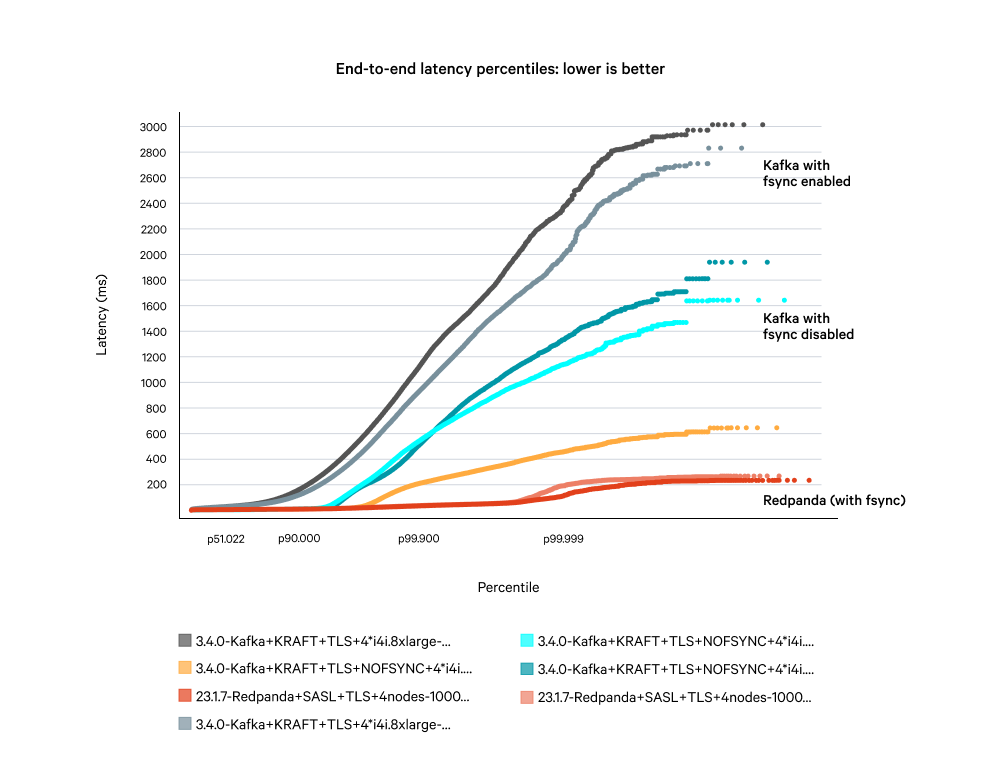
\includegraphics[width=0.75\textwidth]{imgs/fsync.png}
	\captionof{figure}{\href{https://redpanda.com/blog/kafka-kraft-vs-redpanda-performance-2023}{Confronto di latenza tra Kafka e Redpanda con e senza \textit{fsync}.}}
\end{center}




























